\documentclass{beamer}
\usepackage{graphicx}
\title{Towards an AI accelerator implementation using the AHIR-V2 toolset}
\author{Madhav P. Desai \\ Department of Electrical Engineering, IIT Bombay \\ email: madhav@ee.iitb.ac.in}
\begin{document}
\maketitle

\frame{\frametitle{Overview}
\begin{itemize}
\item In its simplest form, an AI accelerator is used for rapid evaluation of the flow of information
through a neural network.  A neural network is characterized by
\begin{itemize}
\item Scale: number of nodes, arcs etc.
\item Topology: connectivity.
\item Computation: the arithmetic used in the network, type of non-linearity.
\end{itemize}
\item Evaluation can be mapped to multi-core, GPU, FPGA, ASIC.
\item Our proposal targets FPGA (and potentially ASIC) implementations.
\end{itemize}
}

\frame{\frametitle{A generic neural network}

\begin{figure}
\centering
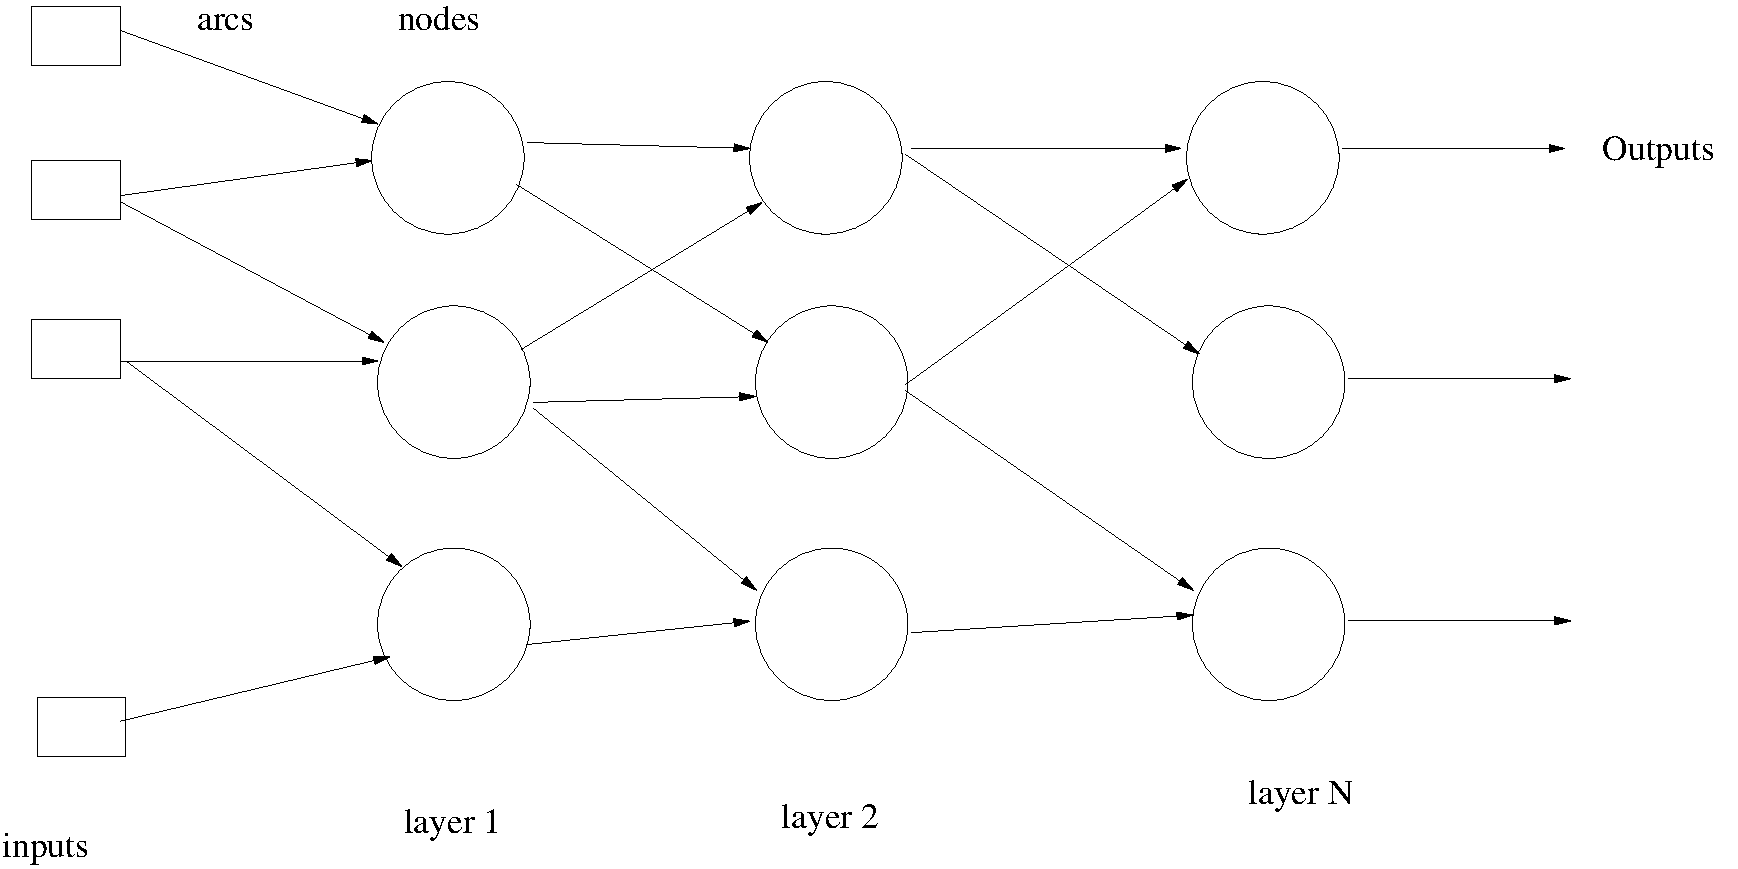
\includegraphics[width=10cm]{figs/GenericNN.pdf}
\caption{A generic neural network}
\label{fig:GenericNN}
\end{figure}
}

\frame[containsverbatim]{\frametitle{Algorithm}
\begin{verbatim}
for L in layers {
   for N in nodes(L) {
       X = getInputs(N)
       Y = evaluate(N,X)
       updateValues (N,Y)
   }
}
\end{verbatim}
}

\frame{\frametitle{Affinity: LDPC decoding}

\begin{figure}
\centering
\includegraphics[width=10cm]{figs/ldpc.pdf}
\caption{LDPC decoding scheme}
\label{fig:ldpc}
\end{figure}

}

\frame{\frametitle{Affinity: parallelization of LDPC decoding}

\begin{figure}
\centering
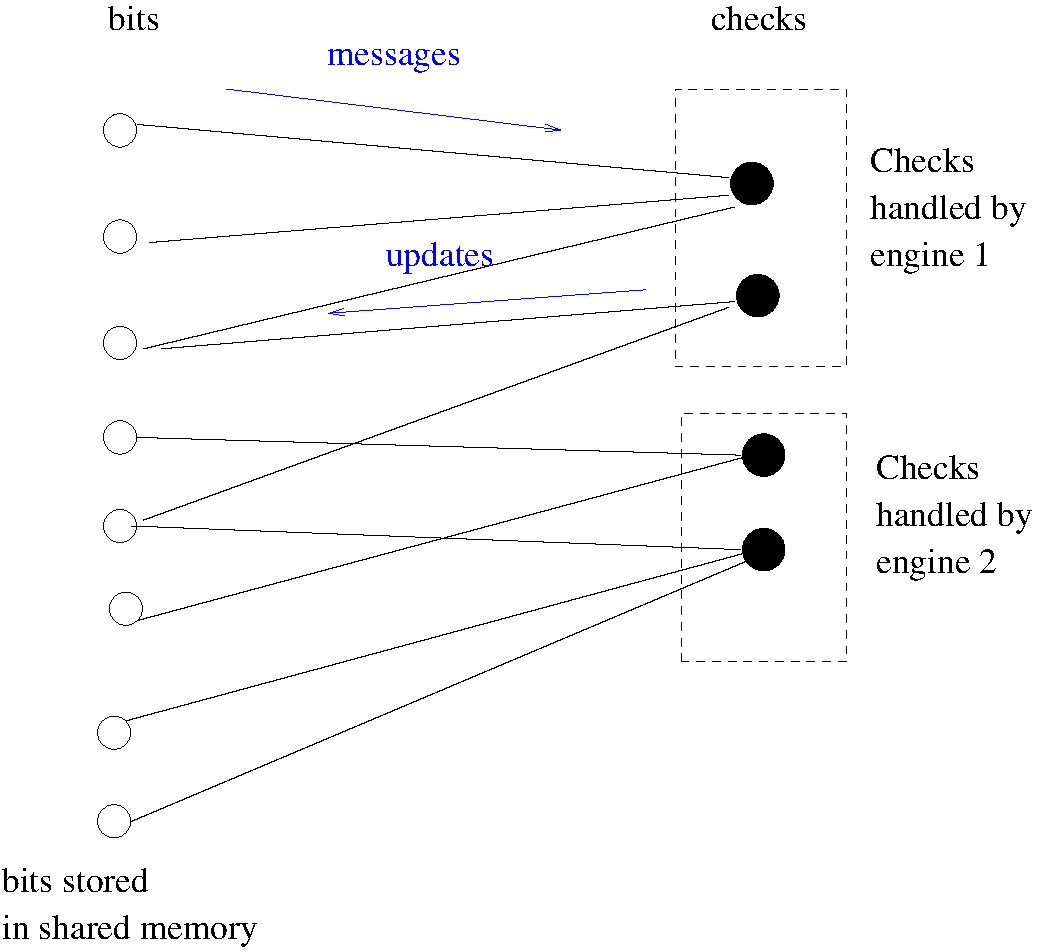
\includegraphics[width=10cm]{figs/parallelization.pdf}
\caption{Parallelization of LDPC decoding scheme}
\label{fig:ldpcPar}
\end{figure}

}

\frame[containsverbatim]{\frametitle{Summary of our work with LDPC decoder}

For 16K point blocks.

\begin{verbatim}
                   FF-count   Memory  Mbps/iteration
Single-engine      12K        148KB   3    Mbps/iteration
Two-engine         17K        148KB   5.8  Mbps/iteration 
Four-engine        33K        148KB   10.2 Mbps/iteration
\end{verbatim}

}

\frame[containsverbatim]{\frametitle{Highlights of our work with LDPC decoder}

\begin{itemize}
\item Ability to handle arbitrary parity check matrix with 16K checks, 16K block size,
max 1024 non-zero entries per row, max number of entries in matrix = 128K.
\item Organization of sparse matrix data into blocks.
\item Use of low precision floating point types.
\item Parallelization using multiple engines, with each engine handling
subset of check nodes.
\item Fast development time using AHIR-V2 toolset.
\begin{verbatim}
-------------------------------------------
lines-of-code
-------------------------------------------
C-model              1976
Aa-model             1598
-------------------------------------------
\end{verbatim}
\end{itemize}

}

\frame[containsverbatim]{\frametitle{What is the AHIR-V2 toolset?}
\begin{itemize}
\item Describe hardware algorithmically.
\begin{itemize}
\item In C.
\item In {\bf Aa}.
\end{itemize}
\item Compiler can translate algorithm into efficient pipelined hardware.
\end{itemize}
}


\frame[containsverbatim]{\frametitle{Example}
\begin{verbatim}
float a[1024], b[1024], c[1024], d[1024];
void foo() {
  int I;
  for (I=0; I < 1024; I++)
  {
     d[I] = (a[I]*b[I]) + c[I]; 
  }
}
\end{verbatim}
}

\frame[containsverbatim]{\frametitle{Translation}

\begin{figure}
\centering
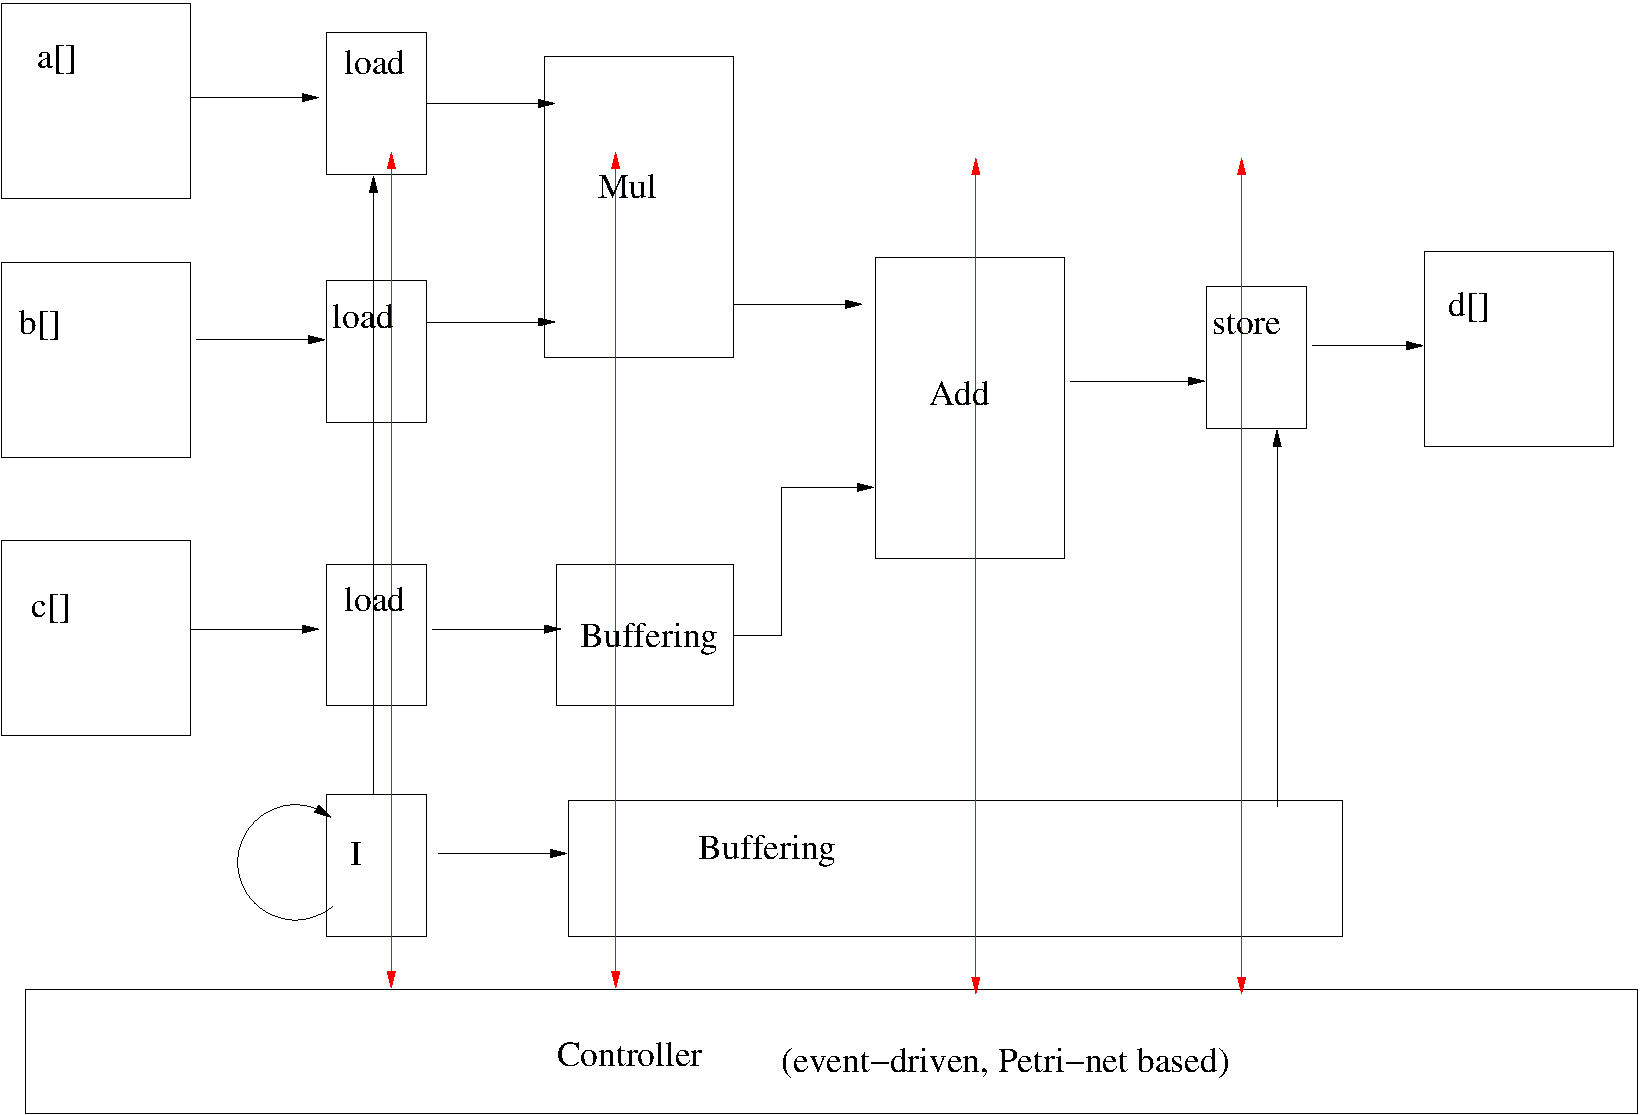
\includegraphics[width=10cm]{figs/AhirSystem.pdf}
\caption{Pipeline generated by the compiler}
\label{fig:AhirSystem}
\end{figure}

}

\frame[containsverbatim]{\frametitle{Success stories: AHIR-V2}
\begin{itemize}
\item Complete 32-bit pipelined processor implementation (AJIT processor, based on SPARC-V8 ISA).
\item Complete NAVIC (GPS+IRNSS) base-band receiver design.
\item LDPC decoder for unstructured parity check matrices (sponsored by Seagate).
\item Competitive, complex and complete designs.
\end{itemize}
}

\frame[containsverbatim]{\frametitle{AHIR-V2: distinguishing features}
\begin{itemize}
\item Algorithm specifies sequencing, not timing.  Functional correctness
is independent of hardware timing.
\item Compiler does not do state enumeration.
\item Generated hardware is self-scheduled (imposes sequence implied by algorithm).
\begin{itemize}
\item Timing optimization is independent of functional correctness.
\end{itemize}
\item Same test setup can be used to verify at the algorithm level and at the hardware level.
\end{itemize}
}

\frame[containsverbatim]{\frametitle{Back to AI: naive parallelization and beyond}

\begin{verbatim}
for L in layers {
   // parallelize
   for N1,N2 in nodes(L) {
       parallel {
          sequence {X1 = getInputs(N1),
                    Y1 = evaluate(N1,X1)}
          sequence {X2 = getInputs(N2),
                    Y2 = evaluate(N2,X1)}
       }
       updateValues (Y1,Y2)
   }
}
\end{verbatim}
}

\frame[containsverbatim]{\frametitle{Options to investigate}
\begin{itemize}
\item Data types (reduced order floats).
\begin{itemize}
\item 16-bit (and smaller) FP format proven in LDPC work.
\end{itemize}
\item SIMD operations (8x8 etc.)
\item Efficient sparse data storage and access.
\begin{itemize}
\item Block based scheme explored in LDPC work.
\end{itemize}
\item Degree of parallelism (limits imposed by Amdahl's law).
\item Explore limits of programmability and flexibility.
\end{itemize}
}

\frame[containsverbatim]{\frametitle{Milestones}

\begin{itemize}
\item Recruitment: 3 Master's students are working on this project.
\item Single engine accelerator (June 2020):
\begin{itemize}
\item data types: 8-bit signed/unsigned int, 16-bit reduced precision float, 32-bit float.
\item weighted sparse graph representation in memory.
\item pipelined evaluation loop.
\item demonstration on FPGA: power, area, performance.
\end{itemize}
\item Multi-engine accelerator (December 2020):
\begin{itemize}
\item Node partitioning across engines.
\item Memory reorganization to reduce conflicts.
\item Scalability studies.
\item demonstration on FPGA: power, area, performance.
\end{itemize}
\end{itemize}

}

\frame[containsverbatim]{\frametitle{Deliverables}
\begin{itemize}
\item Validation of neural network accelerator.
\item Establish limits of approach: capacity, performance, power.
\end{itemize}
}

\frame[containsverbatim]{\frametitle{Looking forward}

\begin{itemize}
\item Possibility of hardware support for online learning.
\item Exploration of daptive system architectures.
\end{itemize}

}

\end{document}
